\documentclass[conference]{IEEEtran}
\IEEEoverridecommandlockouts
% The preceding line is only needed to identify funding in the first footnote. If that is unneeded, please comment it out.
\usepackage{cite}
\usepackage{amsmath,amssymb,amsfonts}
\usepackage{algorithmic}
\usepackage{graphicx}
\usepackage{textcomp}
\usepackage{xcolor}
\usepackage{mathtools}
\usepackage{subfigure}

\def\BibTeX{{\rm B\kern-.05em{\sc i\kern-.025em b}\kern-.08em
    T\kern-.1667em\lower.7ex\hbox{E}\kern-.125emX}}
\begin{document}

\title{Orientation Tracking and Panorama Generation\\

}

\author{\IEEEauthorblockN{1\textsuperscript{st} Pengxi Zeng}
    La Jolla, CA \\
    p2zeng@ucsd.edu}


\maketitle

\begin{abstract}
    This paper presents an approach to solving the Simultaneous Localization and Mapping (SLAM) 
    problem using the Extended Kalman Filter (EKF). The SLAM problem is the task of estimating 
    the position and orientation of a robot as well as the positions of features or landmarks 
    in the environment, while simultaneously building a map of the environment. The EKF is a 
    popular algorithm for estimating the state of nonlinear dynamic systems and is well-suited
    to the SLAM problem due to its ability to handle nonlinear measurement and motion models.
\end{abstract}

\begin{IEEEkeywords}
    SLAM, Extended Kalman Filter
\end{IEEEkeywords}

\section{Introduction}

Simultaneous Localization and Mapping (SLAM) is the problem of estimating the trajectory of a robot and simultaneously building a map of its environment. SLAM is a fundamental problem in robotics and has many applications in autonomous driving, robotics, and augmented reality.

One approach to solving the SLAM problem is to use the Extended Kalman Filter (EKF), which is a popular algorithm for estimating the state of nonlinear dynamic systems. In the context of SLAM, the EKF is used to estimate the pose of the robot (i.e., its position and orientation) as well as the positions of the landmarks in the environment.

The basic idea of EKF-based SLAM is to use sensor measurements (e.g., odometry, laser range-finder data, etc.) to estimate the pose of the robot and update the map of the environment. The EKF operates in a recursive fashion, where it uses the current state estimate and measurements to predict the next state estimate, and then uses this estimate to update the map.

One of the challenges in EKF-based SLAM is that the measurement and motion models are typically nonlinear, which makes it difficult to use the standard Kalman Filter. However, the EKF provides a way to handle nonlinear models by approximating them as linear models around the current state estimate. This allows the EKF to estimate the state of the system even when the models are nonlinear.

Overall, EKF-based SLAM is a powerful approach to solving the problem of robot localization and mapping, and has been successfully used in many real-world applications.


\section{Problem Formulation}
\subsection{General Form}
We usually adopt extened kalman filter to solve SLAM problem. The main difference between common kalman filter and EKF is that
EKF does not require that the model to be linear. In EKF, we assume the prior obeys the normal distribution:
\begin{equation}
    \mathbf{x}_t | \mathbf{z}_{0:t}, \mathbf{u}_{0:t-1} \sim N (\mu_{t|t}, \Sigma_{t|t})
\end{equation}

And the motion model and observation model could be described respectively as follows:
\begin{equation}
    \begin{aligned}
    & \mathbf{x}_{t+1}=f\left(\mathbf{x}_t, \mathbf{u}_t, \mathbf{w}_t\right), \quad \mathbf{w}_t \sim \mathcal{N}(\mathbf{0}, W) \\
    & F_t:=\frac{d f}{d \mathbf{x}}\left(\boldsymbol{\mu}_{t \mid t}, \mathbf{u}_t, \mathbf{0}\right), \quad Q_t:=\frac{d f}{d \mathbf{w}}\left(\boldsymbol{\mu}_{t \mid t}, \mathbf{u}_t, \mathbf{0}\right)
    \end{aligned}
\end{equation}

\begin{equation}
    \begin{aligned}
    & \mathbf{z}_t=h\left(\mathbf{x}_t, \mathbf{v}_t\right), \quad \mathbf{v}_t \sim \mathcal{N}(\mathbf{0}, V) \\
    & H_t:=\frac{d h}{d \mathbf{x}}\left(\boldsymbol{\mu}_{t \mid t-1}, \mathbf{0}\right), \quad R_t:=\frac{d h}{d \mathbf{v}}\left(\boldsymbol{\mu}_{t \mid t-1}, \mathbf{0}\right)
    \end{aligned}
\end{equation}


Thus, from the motion model, we could do the prediction and update step as follows:


\begin{equation}
    \begin{aligned}
    & \mu_{t+1 \mid t}=f\left(\mu_{t \mid t}, \mathbf{u}_t, \mathbf{0}\right) \\
    & \Sigma_{t+1 \mid t}=F_t \Sigma_{t \mid t} F_t^{\top}+Q_t W Q_t^{\top} 
    \end{aligned}
\end{equation}

\begin{equation}
    \begin{aligned}
    & \mu_{t+1 \mid t+1}=\mu_{t+1 \mid t}+K_{t+1 \mid t}\left(z_{t+1}-h\left(\mu_{t+1 \mid t}, 0\right)\right) \\
    & \Sigma_{t+1 \mid t+1}=\left(I-K_{t+1 \mid t} H_{t+1}\right) \Sigma_{t+1 \mid t}
    \end{aligned}
\end{equation}
in which the Kalman gain could be calculated as:
\begin{equation}
    \begin{aligned}
    K_{t+1 \mid t}:=&\Sigma_{t+1 \mid t} H_{t+1}^{\top} \\ &\left(H_{t+1} \Sigma_{t+1 \mid t} H_{t+1}^{\top}+R_{t+1} V R_{t+1}^{\top}\right)^{-1}
    \end{aligned}
\end{equation}



\section{Technical Approach}
\subsection{Pose Prediction}
Consider the localization-only problem, from the motion model, we know the funtion of calculating the pose with twist:
\begin{equation}
T_{k+1} = T_k\exp{\tau_k\hat{\zeta}_k}
\end{equation}

Then the nominal and perturbation could be calculated as:
\begin{equation}
    \begin{aligned}
    \boldsymbol{\mu}_{t+1} & =\boldsymbol{\mu}_t \exp \left(\tau_t \hat{\mathbf{u}}_t\right) \\
    \delta \boldsymbol{\mu}_{t+1} & =\exp \left(-\tau_t \hat{\mathbf{u}}_t\right) \delta \boldsymbol{\mu}_t+\mathbf{w}_t
    \end{aligned}
\end{equation}

And the covariance is:
\begin{equation}
    \begin{aligned}
    &\Sigma_{t+1 \mid t} =\mathbb{E}\left[\delta \boldsymbol{\mu}_{t+1 \mid t} \delta \boldsymbol{\mu}_{t+1 \mid t}^{\top}\right] \\
    &=\exp \left(-\tau \hat{\mathbf{u}}_t\right) \Sigma_{t \mid t} \exp \left(-\tau \hat{\mathbf{u}}_t\right)^{\top}+W
    \end{aligned}
\end{equation}

\subsection{Update}
\subsubsection{Mapping Update}
Since we assume all the features stay static, we don't need to predict the features' poses. The update for the landmarks' 
positions could be formulated as:
\begin{equation}
    \begin{aligned}
    K_{t+1} & =\Sigma_t H_{t+1}^{\top}\left(H_{t+1} \Sigma_t H_{t+1}^{\top}+I \otimes V\right)^{-1}, \\
    \mu_{t+1} & =\mu_t+K_{t+1}\left(\mathbf{z}_{t+1}-\tilde{\mathbf{z}}_{t+1}\right), \\
    \Sigma_{t+1} & =\left(I-K_{t+1} H_{t+1}\right) \Sigma_t,
    \end{aligned}
\end{equation}
where $H_{t+1, i, j} = \mathbb{I}(\Delta_t(j) = i) K_s \frac{d\pi}{d\mathbf{q}}(_{o}T_{w}\underline{\mu}_{t,j})P^{\top}$

\subsubsection{Pose Update}
The two differences between mapping update and pose update are how to calculate $H_{t+1}$ and the rule for mean:
\begin{equation}
    H_{t+1, i}=-K_s \frac{d \pi}{d \mathbf{q}}\left( _oT_i \boldsymbol{\mu}_{t+1 \mid t}^{-1} \underline{\mathbf{m}}_j\right) \prescript{}{o}{T_i}\left(\boldsymbol{\mu}_{t+1 \mid t}^{-1} \underline{\mathbf{m}}_j\right)^{\odot}
\end{equation}
\begin{equation}
    \mu_{t+1} =\mu_t\exp\left((K_{t+1}\left(\mathbf{z}_{t+1}-\tilde{\mathbf{z}}_{t+1}\right)\hat)\right)
\end{equation}

\subsubsection{Simultaneously Update}
The former two updates both assume other contions are correct and static. However, in SLAM, this could lead to a problem that 
the pose and the landmarks are correlated in the process. And the former two updates would lose the covariance information
between the pose and the landmarks.

\subsection{Some More Details}
\textbf{The initialization of $\boldsymbol{q}_T$}: considering the fact that $\boldsymbol{q}_T$ is initialized using
motion model, the loss related to motion model is very small at first, and the gradient could become NAN. Thus, when
initializing $\boldsymbol{q}_T$, we added a small noise to it in order to make it bias from original value, so that
NAN would not appear at the start and could better train the model.

\textbf{Training}: when training the model, though we added a noise to $\boldsymbol{q}_T$ in initialization, the loss of
the motion model is still very small. To balance the two loss a little bit, we multiplied the motion loss by 10.

\textbf{Panorama}: when generating panorama, we changed the shape of the coordinates to $[3 \times (r \times c)]$ for
acceleration of the calculation.


\section{Results}
\subsection{Orientation Tracking}
From the results, we can find out that for most of the datasets, angles of Roll and Pitch match with real data realtively
well, but for Yaw, the shape of optimized results match with that of the real data, while the is a gap between them. One
guess is that the accumulation of the error in Yaw could not be well eliminated.

\subsection{Panorama}
From the results we can tell that the pictures have the consistency in space, e.g. the connection of the handrail.

% \begin{figure}[htbp]
%     \centering
%     \subfigure[Roll for Dataset 1]{
%         \begin{minipage}[t]{1\linewidth}
%             \centering
%             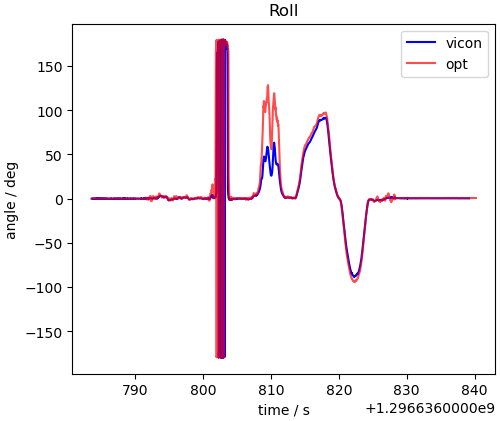
\includegraphics[width=2.5in]{../figs/Roll_1.png}
%             % \caption{}
%         \end{minipage}%
%     }%

%     \subfigure[Pitch for Dataset 1]{
%         \begin{minipage}[t]{1\linewidth}
%             \centering
%             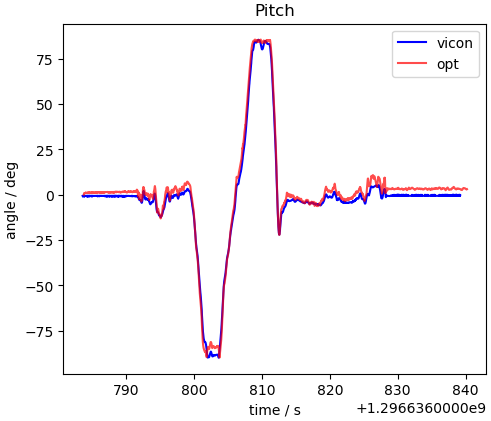
\includegraphics[width=2.5in]{../figs/Pitch_1.png}
%             % \caption{}
%         \end{minipage}
%     }%

%     \subfigure[Yaw for Dataset 1]{
%         \begin{minipage}[t]{1\linewidth}
%             \centering
%             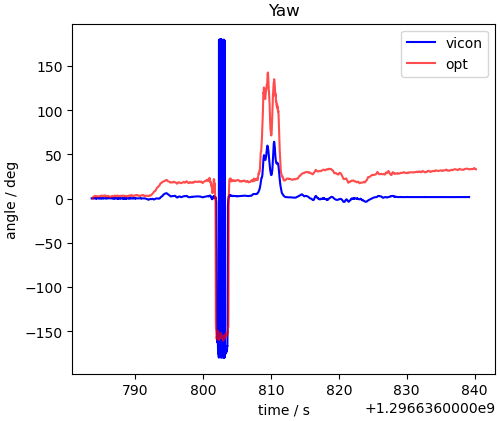
\includegraphics[width=2.5in]{../figs/Yaw_1.png}
%             % \caption{}
%         \end{minipage}
%     }%

%     \subfigure[Panorama for Dataset 1]{
%         \begin{minipage}[t]{1\linewidth}
%             \centering
%             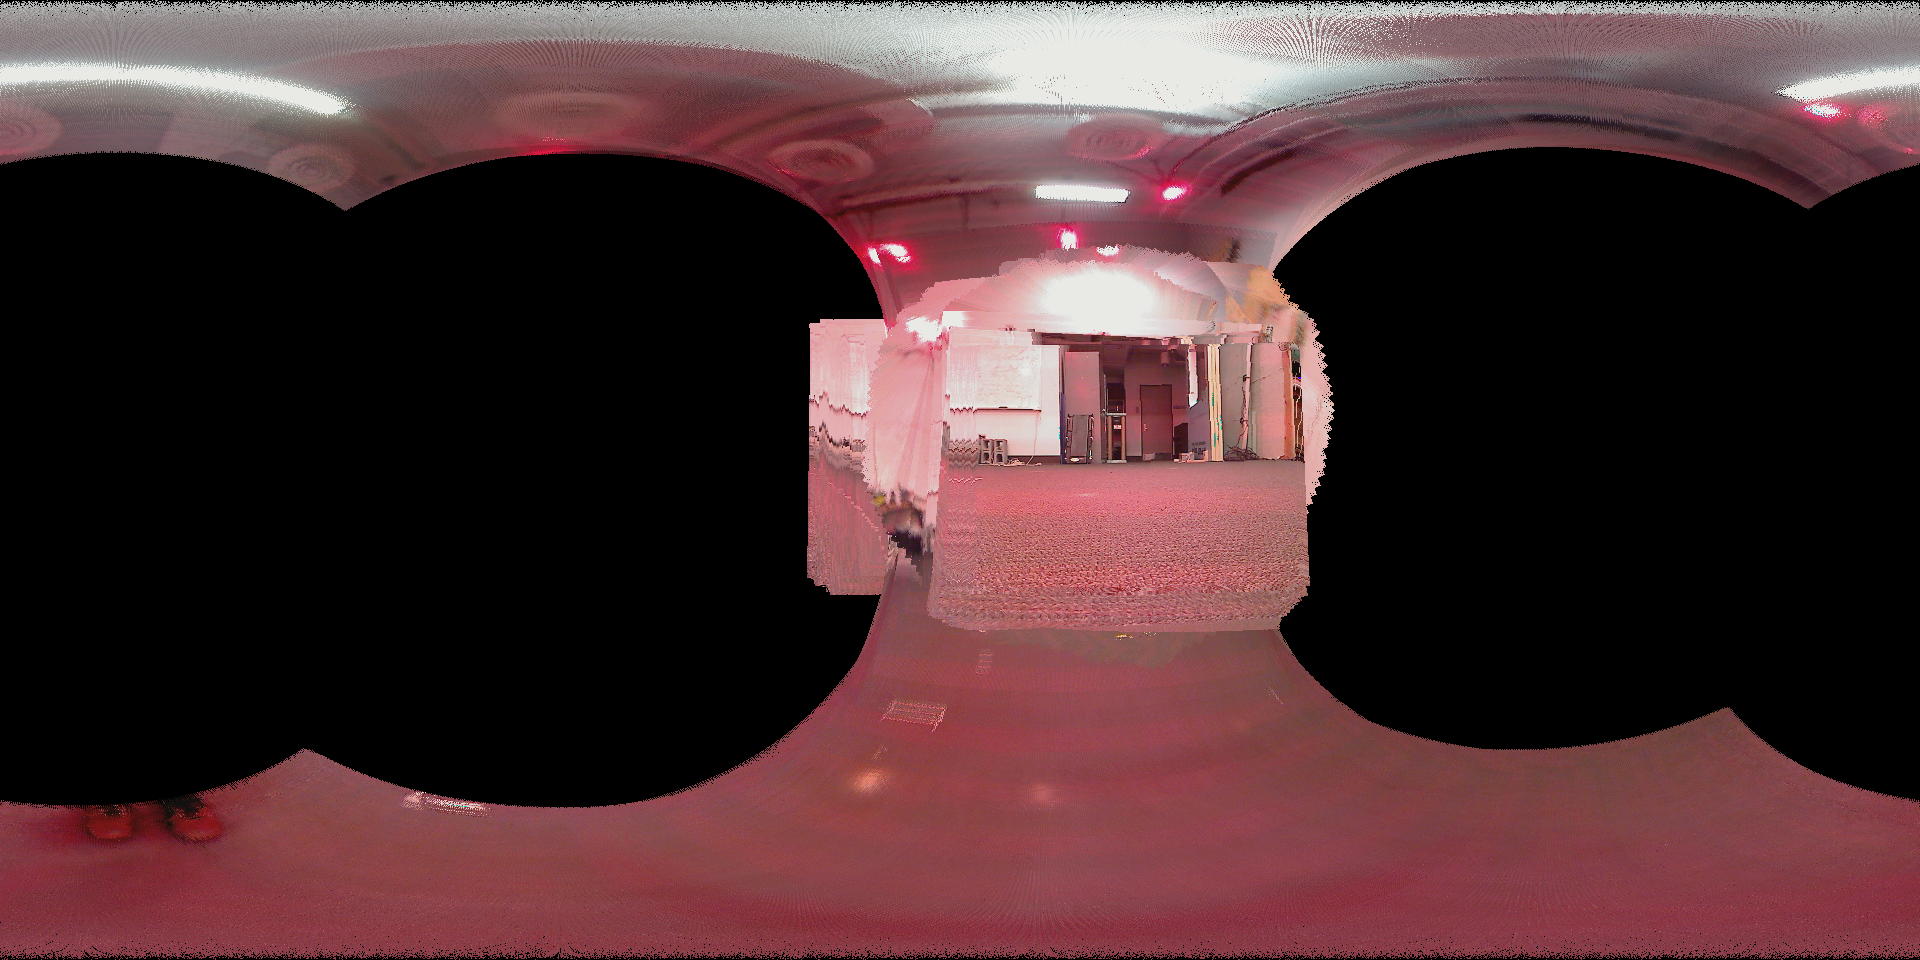
\includegraphics[width=2.5in]{../figs/panorama_1.png}
%             % \caption{}
%         \end{minipage}
%     }%
%     \centering
%     \caption{ Result for Dataset 1}
% \end{figure}

\end{document}
